\documentclass[11pt,spanish]{article}
\usepackage{graphicx}
\usepackage[left=1.3in, right=1.3in, top=1in, bottom=1in]{geometry}
\usepackage[utf8]{inputenc}
\usepackage[noend,ruled,linesnumbered,spanish]{algorithm2e}
\usepackage{forest,adjustbox}
\usepackage{babel}
\title{Tarea III\\ \small{Análisis de Algoritmos, Grupo 3}}
\author{
Maria Andrea Rodriguez Tastets$^{1}$, Erick Elejalde Sierra$^{2}$,\\ Cristóbal Donoso Oliva$^{3}$ Matías Medina Silva$^{4}$\\\\
\small{$^{1}$Docente a cargo de la asignatura $^{2}$Ayudante de asignatura}\\
\small{$^{3-4}$Estudiantes de pregrado}\\
\small{$^{1}$andrea@udec.cl $^{2}$erick.elejalde@gmail.com $^{3}$cdonoso94@gmail.com }\\
\small{$^{4}$matiasdmedina@udec.cl}\\
\small{$^{1-2-3-4}$Dpto. de Ingeniería Civil Informática y Ciencias de la Computación}\\
\small{Universidad de Concepción, Concepción, Chile.}\\
}
\date{21 de Junio del 2016}
\begin{document}
\maketitle
\newpage
\tableofcontents
\newpage
\section{Problema del peso disidente}
Asuma que tiene $n$ objetos que tiene peso idéntico, excepto para uno que es un poco más pesado que los otros. Usted tiene una balanza, se puede colocar 2 personas en la balanza y la idea es encontrar el objeto más pesado con el mínimo número de usos de la balanza. Encuentre el lower bound para este problema.
\subsection{Lower Bound}
Primero debemos considerar que la balanaza no es más que la representación de comparar dos objetos $n_i$ $R$ $n_{i+1}$. Así mismo, el peso de cualquier objeto estará determinado por:
\begin{center}$Peso Objeto = Peso Balanza - Peso persona$\end{center}
No sabemos cual es el peso de las personas que están en la balanza, no obs-tante, podemos obviar sus pesos ya que solo nos interesa encontrar el objeto mas pesado.\\\\Para este problema trabajaremos con un \emph{arbol de decisión} describiendo en él todas las posibilidades al momento de comparar.
\tikzset{
    every label/.append style={font=\scriptsize},
    my edge labels/.style={font=\scriptsize},
    dominant/.append style={label=below:$dominant$},
  }
\begin{figure}[h]
\begin{center}  \begin{forest}
    for tree={
      circle,
      draw,
      minimum width=0.5em,
      l sep+=1.0em,
      s sep+=1em,
      anchor=center,
      edge path={
        \noexpand\path[\forestoption{edge}](!u.parent anchor)--(.child anchor)[		my edge labels]\forestoption{edge label};
      },
    },
    delay={
      where n=1{
        edge label/.wrap 2 pgfmath args={
          node[midway, left]{}}{level}{n}
      }{
        edge label/.wrap 2 pgfmath args={
          node[midway, right]{}}{level}{n}
      },
    }
    [$<$, 
       [si, 
       		[,phantom]
       ]
       [$<$, 
        [si, 
        	[,phantom]
        ]
        [$<$,
        	[si,
        		[,phantom]
        	]
        	[$<$,
        	]
        ]
       ]
      ]
    ]
  \end{forest}\end{center}
  \caption{No se que va acá}
   \label{fig:arbol}
  \end{figure}
Notémos que en el peor de los casos necesitaremos $n-1$ comparaciones para encontrar el objeto de mayor peso (altura del árbol). Por lo tanto, se infiere que el \emph{Lower Bound} asociado a este problema es $O(n)$.

\subsection{Demostración}
Imaginemos que exíste un Lower Bound menor de $n-2$ comparaciones. Entonces, existe un objeto el cual no es comparado con su sucesor.\\Consiederemos una entrada de $n$ objetos iguales, esto es: 
\begin{center}$o_0 = o_1 = o_2 = o_3 = ... = o_n$\end{center}
Si agregamos un \emph{nuevo elemento distint}o nuestro algoritmo \textbf{X }debería encontrar la respuesta correcta en $n-2$ comparaciones\\
\begin{center}$o_1...0_n$ $\cup$ $o_{n+1}$\end{center}
Sin embargo, el algoritmo retornaría una respuesta errada ya que siempre dejará un elemento sin verificar y esto trae como consecuencia la discriminación de objetos en el peor de los casos.\\\\Finalmente podemos afirmar que el Lower Bound adecuado al \emph{mejor peor caso} toma un numero lineal de comparaciones, lo que se traduce a la cantidad mínima de usos de balanza O(n).

\section{Hormigas en un palo}
\subsection{Definición del problema}
Un ejército de hormigas camina en un palo horizontal de largo \emph{l}, cada una a una velocidad constante \emph{v}. Cuando una hormiga alcanza el final del palo se cae. Cuando dos hormigas se encuentran ellas se dan vuelta y caminan en sentido contrario. Se sabe la posición inicial de las hormigas pero no su dirección de movimiento. Se te pide determinar el menor y mayor tiempo posible para que todas las hormigas se caigan del palo.\\\\Supongamos que tenemos un conjunto ordenado S = \{a$_{1}, \dots ,a_{n}$\} de n hormigas y un palo de largo \emph{l}. Cada hormiga a$_{i}$ tiene una posición incial p$_{i}$, donde 0 $\leq $ p$_{i}$ $\leq $ \emph{l}.
\subsection{Subestructura óptima}
Antes de definir la subescructura óptima se analizará que sucede cuando dos hormigas colisionan.
\begin{figure}[h]
    \centering
    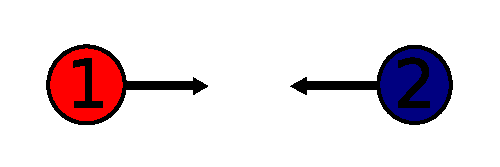
\includegraphics{hormigas1.pdf}
    \caption{Antes de colisión}
    \label{fig:antes}
\end{figure}
\begin{figure}[h]
    \centering
    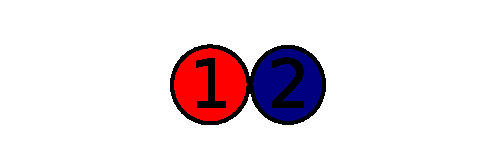
\includegraphics{hormigas2.pdf}
    \caption{Colisión}
    \label{fig:durante}
\end{figure}
\begin{figure}[h]
    \centering
    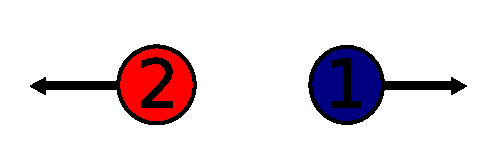
\includegraphics{hormigas3.pdf}
    \caption{Después de colisión}
    \label{fig:despues}
\end{figure}
\\\\\\\\
Como vemos en la figura~\ref{fig:despues}, lo que le sucede a una hormiga tras una colisión es lo mismo que le sucedería a la otra hormiga, en otras palabras, es como si no hubiese habido un choque y las hormigas intercambiarán su ``identidad'', siendo esta representada por los números. Entonces el tiempo total para que todas las hormigas caigan estaría dado por la hormiga que demore más tiempo en cruzar el palo como si no hubiesen colisiones\\\\Denotemos el conjunto S$_{i,j}$ que contiene desde las hormiga \emph{i} hasta la hormiga \emph{j}.\\\\Se asume que el conjunto está ordenado en orden creciente en terminos de \emph{p}, es decir que $\forall$ a$_{k}$ $\in$ S$_{i,j}$ , p$_{k}$ $\leq$ p$_{k+1}$ con 0 $\leq$ i $\leq$ k $\leq$ j, entonces, para encontrar el tiempo máximo es trivial, ya que solo se necesita comparar la horgmia a$_{0}$ con la hormiga a$_{n}$ y calcular cual demoraría más en cruzar a la orilla opuesta del palo. Para el tiempo mínimo, el problema se transofrma en encontrar la hormiga que se demora más tiempo en cruzar el palo, considerando la dirección de movimiento hacia la orilla más cercana.\\\\Luego se tiene un problema S$_{i,j}$, donde una solución a S$_{i,j}$ sería dado por el tiempo mínimo de la hormiga a$_{k}$, tal que p$_{i}$ $\leq$ p$_{k}$ $\leq$ p$_{j}$. Esto genera dos subproblemas S$_{i,k}$ y S$_{k+1,j}$, donde la solución al problema S$_{k+1,j}$ debe ser menor que a$_{k}$.\\\\La subestructura óptima es la siguiente. Suponemos que una solucion A$_{i,j}$ de S$_{i,j}$ es el tiempo mínimo de la hormiga a$_{k}$. Entonces las soluciones A$_{i,k}$ de S$_{i,k}$ y A$_{k+1,j}$ de S$_{k+1,j}$ que se usan en la solución optima de S$_{i,j}$ deben ser óptimas.
\subsection{Demostración subestructura óptima}
Se asume que A$_{i,j}$ (el tiempo mínimo de la hormiga a$_{k}$) es la solución óptima del problema S$_{i,j}$. Si hay una solución A'$_{i,k}$ de S$_{i,k}$ con una hormiga que tome más tiempo en cruzar el palo que en A$_{i,k}$, entonces podríamos reemplazar A$_{i,k}$ por A'$_{i,k}$ en A$_{i,j}$ y así mismo reemplazar A'$_{i,k}$ por A$_{i,j}$, ya que a$_{k}$ $\in$ S$_{i,k}$. Ya que asumimos que A$_{i,j}$ era una solución optima, entonces hay una contradicción. Lo mismo se aplica para S$_{k,j}$
\subsection{Solución recursiva}
Se quiere encontrar el tiempo de la hormiga a$_{k}$ que demore más en recorrer el palo teniendo en cuenta la opción minima, es decir, que camine hacia la orilla más cercana. Para el calculo de la opción minima se definió la siguiente función d[i] considerando la posición p${i}$, el largo del palo \emph{l} y la velocidad \emph{v}:\\
\begin{figure}[h]
\begin{center}
$d[i] = min\{\frac{l - p{i}}{v},\frac{p{i}}{v}\}$
\caption{Función de opción mínima}
\label{fig:opmin}
\end{center}
\end{figure}
\\\\
Luego, denotamos c[i,j] como el tiempo de la hormiga que más tiempo demora en cruzar el palo considerando su opción mínima:\\
\begin{figure}[h]
\begin{center}$c[i,j] = \left\{
\begin{array}{c l}  
  0 & S_{i,j} = 0\\
  d[i] & S_{i,j} = 1\\
  max \{c[i,\lfloor(i+j)/2\rfloor],c[\lfloor(i+j)/2\rfloor,j]\} & S_{i,j} \neq 0
\end{array}
\right.
$
\caption{Tiempo de caida}
\label{fig:opmin}\end{center}
\end{figure}
\subsection{Elección Greedy}
Supongamos que $A_{i,j}$ es la solución óptima al problema y por lo tanto se compone de $I_1$\dots$I_k$ instancias. La solución estará definida por la comparación de todas las posiciones de una partición, y de esta forma determinar el máximo de los valores mínimos asociados a la distancia de una hormiga(ver figura~\ref{fig:opmin}).\\\\La opción Greedy será particionar el conjunto $S_{i,j}$ por la mitad $\lfloor\frac{i+j}{2}\rfloor = k$, por lo tanto, quedarán dos particiones $S_{i,k}$ y $S_{k+1,j}$. Luego comparamos las hormigas $a_k$ y $a_{k+1}$ las cuales son las más próximas a la mitad y nos quedamos con la hormiga a$_{c}$ más cercana a la mitad del palo $l$. Dicho de otra forma:

\begin{center} $a_{c} = min\{|l/2-p_k|,|l/2-p_{k+1}|\}$\end{center}
Luego consideramos la partición que contenga a$_{c}$ y descartamos el conjunto de hormigas de la otra partición. Finalmente, iteramos hasta encontrar la hormiga que esté más cerca de la mitad $l/2$,
\subsection{Teorema y demostración elección Greedy}
\subsubsection{Teorema}
Se considera un subproblema S$_{k}$ no vacío y dos particiones S$_{m}$ y S$_{h}$ de S$_{k}$, sea a$_{k}$ la hormiga que toma más tiempo en llegar a la orilla considerando la dirección mínima perteneciente a S$_{k}$. Entonces dependiendo de la elección, es decir si se elige la partición S$_{m}$ ó S$_{h}$, a$_{k}$ $\in$ S$_{m}$ ó a$_{k}$ $\in$ S$_{h}$.
\subsubsection{Demostración}
Sea A$_{k}$ la hormiga con mayor tiempo en el conjunto S
\subsection{Algoritmo recursivo}
En este algoritmo el arreglo S representa las posiciones iniciales de las hormigas ordenadas de forma decreciente, L el tamaño del palo y V la velocidad de las hormigas e i,j son los indices de la partición.\\\\
\begin{algorithm}[H]
 \KwData{S[0 $\dots$ n],L,V,i,j}
 \KwResult{Tiempo mínimo en que todas las hormigas caen}
 k = (i+j)/2\;
 medio = L/2\;
 \eIf{i $=$ j }{
 	\eIf{(L - S[i]) $\leq$ S[i]}{
 		\textbf{return} (L - S[i])/V\;
 	}{
 		\textbf{return} S[i]/V\;
 	}
 	
 	
 }{
 	\eIf{$|$ medio - S[k] $|$ $\leq$ $|$ medio - S[k+1] $|$}{
 		\textbf{return} TMHrecursivo(S,L,V,i,k)\;
 	}{
 		\textbf{return} TMHrecursivo(S,L,V,k+1,j)\;
 	}
 } 
 \caption{TMHrecursivo}
 \label{fig:algo1}
\end{algorithm}
\subsection{Algoritmo iterativo}
Este algoritmo recibe los mismo parámetros que el algoritmo recursivo y hace lo mismo de forma iterativa.\\\\
\begin{algorithm}[H]
 \KwData{S[0 $\dots$ n],L,V,i,j}
 \KwResult{Tiempo mínimo en que todas las hormigas caen}
 k = (i+j)/2\;
 medio = L/2\;
 \While{i $\neq$ j}{
 	k = (i+j)/2\;
 	\eIf{$|$ medio - S[k] $|$ $\leq$ $|$ medio - S[k+1] $|$}{
 		j = k\;
 	}{
 		i = k+1\;
 	}
 }
 \eIf{(L - S[i]) $\leq$ S[i]}{
 		\textbf{return} (L - S[i])/V\;
 	}{
 		\textbf{return} S[i]/V\;
 	}
 \caption{TMHiterativo}
 \label{fig:algo2}
\end{algorithm}
\end{document}